\begin{tikzpicture}
\begin{axis}[
  width=0.78\linewidth, height=5.4cm,
  xmin=-0.05, xmax=1.62, ymin=-1.4, ymax=10.5,
  xlabel={$s$}, ylabel={weighted gap $\Delta(s)\ \ (\times10^{-4})$},
  xtick={0,0.5,0.75,1,1.25,1.5},
  xticklabels={$0$,$\tfrac12$,$\tfrac34$,$1$,$\tfrac54$,$\tfrac32$},
  axis lines=left,
  legend style={font=\scriptsize, draw=none, at={(0.5,-0.32)}, anchor=north, legend columns=2, /tikz/every even column/.append style={column sep=8pt}},
  legend cell align=left,
  tick label style={font=\scriptsize}, label style={font=\small},
]
  \addplot[black, thick, domain=-0.05:1.62, samples=2] {0};
  \addlegendentry{common future law (Prop.~\ref{prop:zero-gap})}
  \addplot[black!55, densely dashed, domain=-0.05:1.62, samples=2] {0.4};
  \addlegendentry{level $1/25000$}
  \addplot[only marks, mark=*, mark size=1.7pt, black] coordinates {
    (0,0) (0.5,9.252) (0.75,8.839) (1,5.749) (1.25,0.819) (1.5,5.152)};
  \addlegendentry{correlated law, $q^{(1)}$}
  \addplot[only marks, mark=o, mark size=2.3pt, black] coordinates {
    (0,0) (0.5,9.119) (0.75,8.638) (1,5.481) (1.25,0.485) (1.5,5.554)};
  \addlegendentry{correlated law, $q^{(2)}$}
  \draw[|-|, black!70] (axis cs:1.25,-0.85) -- node[below, font=\scriptsize]{a zero of $\Delta$} (axis cs:1.5,-0.85);
\end{axis}
\end{tikzpicture}
